% TeX root=../main.tex

\settrimmedsize{\stockheight}{\stockwidth}{*}
\settypeblocksize{220mm}{130mm}{*}
\setlrmargins{*}{*}{1.7}
\setulmargins{30mm}{*}{*}
\setmarginnotes{20pt}{100pt}{10pt}
\checkandfixthelayout%

% \setsidefeet{\marginparsep}{\marginparwidth}%
% {0.8\onelineskip}{0pt}%
% {\normalfont\footnotesize}{\textheight}%
\setsidecaps{\marginparsep}{\marginparwidth}
\setlength{\footmarkwidth}{0.5em}
\setlength{\footmarksep}{0em}
\setlength{\footparindent}{0em}
\footmarkstyle{\textsuperscript{#1}\hspace{0.5em}}

\makeoddfoot{plain}{}{}{\thepage}
\makeevenfoot{plain}{\thepage}{}{}
\makepagestyle{ruled}
\makeevenfoot{ruled}{\thepage}{}{} % page numbers at the outside
\makeoddfoot{ruled}{}{}{\thepage}
\makeheadrule{ruled}{\textwidth}{0.75pt}
\makeevenhead{ruled}{\scshape\leftmark}{}{}
\makeoddhead{ruled}{}{}{\scshape\rightmark}
\makepsmarks{ruled}{%
	\nouppercaseheads%
	\createmark{chapter}{left}{shownumber}{\scshape}{.\space}
	\createmark{part}{right}{shownumber}{}{.\space}
	\createmark{section}{right}{shownumber}{}{.\space}
	\createmark{subsection}{right}{shownumber}{}{.\space}
	\createplainmark{toc}{both}{\contentsname}
	\createplainmark{lof}{both}{\listfigurename}
	\createplainmark{lot}{both}{\listtablename}
	\createplainmark{bib}{both}{\bibname}
	\createplainmark{index}{both}{\indexname}
	\createplainmark{glossary}{both}{\glossaryname}
}

% Decorando divisões
\chapterstyle{hangnum}
\setsecnumdepth{subsection}
\setcounter{tocdepth}{3}
\newcommand\chap[1]{%
	\chapter*[#1]{#1}%
	\addcontentsline{toc}{chapter}{#1}}


% Paleta de cores
\usepackage{xcolor}
\definecolor{green}{RGB}{16,87,87} % rgb(16,87,87)
\definecolor{red}{RGB}{193, 11, 105} % rgb(193, 11, 105)
\definecolor{yellow}{RGB}{218,222,104} % rgb(218,222,104)
\definecolor{pink}{RGB}{243,179,145} % rgb(243,179,145)
\definecolor{blue}{RGB}{161,184,206} % rgb(161,184,206)

\usepackage[tracking=true]{microtype}

\newcommand{\colofao}[0]{
	\pagestyle{empty}
	\cleartoevenpage%
	\hfill
	\vfill
	\begin{adjustwidth}{5em}{5em}
		\begin{center}
			\noindent Esse documento foi diagramado usando o sistema
			\href{https://lualatex.org}{Lua\TeX} mantido por Manuel
			Pégourié-Gonnard. Todos os \emph{softwares} utilizados na
			diagramação deste document são gratuitos e \emph{open source}.\par
			{\today.}
		\end{center}
	\end{adjustwidth}
	\bigskip
	\noindent
}

\newcommand{\thecoverpage}{
	{
			\thispagestyle{empty}
			\flushright%
			\AddToShipoutPictureFG*{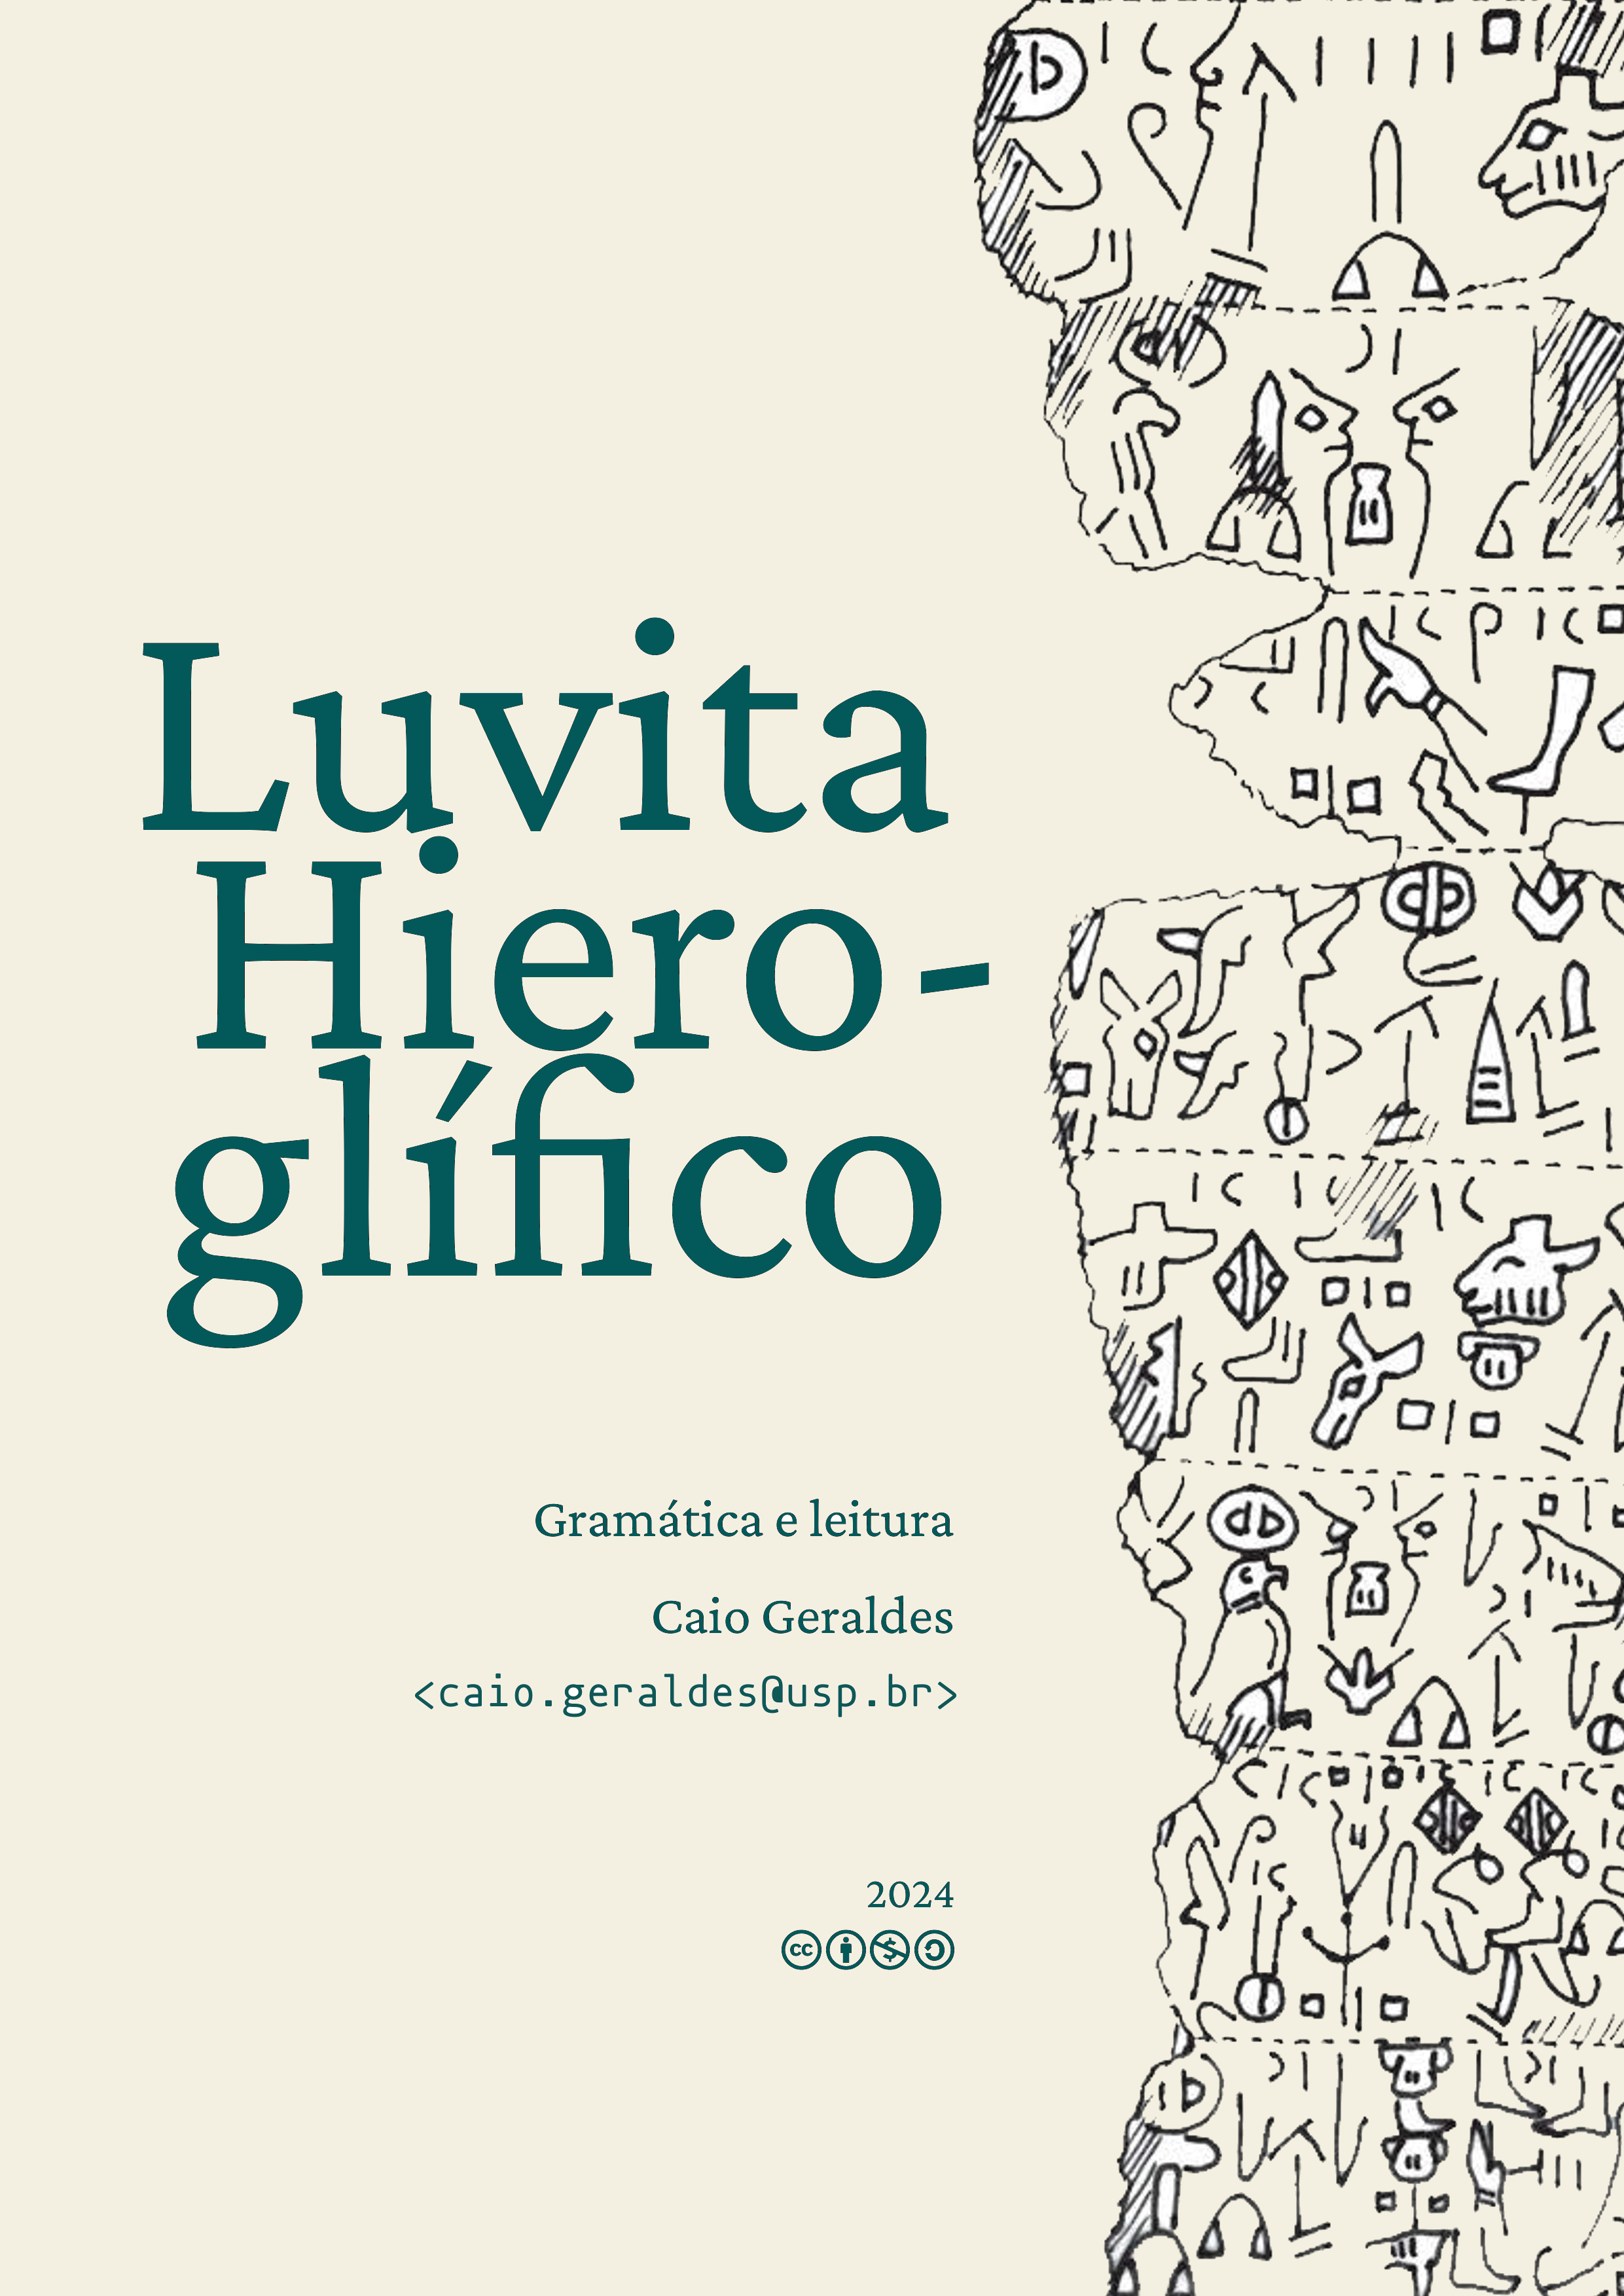
\includegraphics[width=\paperwidth, height=\paperheight]{../../../Mídia/capa.png}}
			\vspace*{45mm}
			\noindent {\scalefont{10}\thetitle}
			\vfill


			\noindent\scalefont{1.7}Gramática e leitura

			\vspace{0.75\onelineskip}

			\noindent\theauthor%

			\vspace{0.5\onelineskip}

			\noindent\scalefont{0.8}\href{mailto:caio.geraldes@usp.br}{\texttt{<caio.geraldes@usp.br>}}


			\vfill{}
			2024\\
			\ccbyncsa

		}
}


\newcommand{\thetitlepage}{
	{
			\thispagestyle{empty}
			\flushright%
			\vspace*{45mm}
			\noindent {\scalefont{10}\thetitle}
			\vfill


			\noindent\scalefont{1.7}Gramática e leitura

			\vspace{0.75\onelineskip}

			\noindent\theauthor%

			\vspace{0.5\onelineskip}

			\noindent\scalefont{0.8}\href{mailto:caio.geraldes@usp.br}{\texttt{<caio.geraldes@usp.br>}}


			\vfill{}
			2024\\
			\ccbyncsa

		}
}

\usepackage{scalefnt}
\pagestyle{companion}
